\section{Reflection security}\label{sec:refsec}

We now define the theoretical model for reflection attacks. We propose a
cryptographic game for a simulation-based model and present proofs of insecurity
under the necessary assumptions. We then move on to describe the properties of
the various elements in the game and describe existing compression attacks,
including Rupture, as instances of the theoretical model we introduce.

\subsection{The reflection game}\label{subsec:refsecgame}

Let $\mathcal{T} = (Gen, K, \mathcal{D})$ be a triplet of algorithms. In this
triplet, $Gen$ is a key generation algorithm which, given a security parameter
$1^\lambda$ returns some key $\kappa$. The function $K$ is an encryption
function with three parameters: The key $\kappa$ and two plaintexts $s$ and $r$,
which we call the \textit{secret} and \textit{reflection} specifically. For now,
we leave the question of how these plaintexts are combined to be encrypted
together undefined; this will be instantiated into a concrete function when we
discuss the security of particular schemes.

Let $\mathcal{A}$ be an adversary and $\mathcal{S}$ be a simulator. Also let
$\mathcal{M}$ be a distribution of plaintexts and $g$ a function defined on its
support, as well as some function $Com(\cdot)$ defined on the domain of $K$. We
call $Com$ the compression function and require that it is a deterministic
polynomially computable and reversible bijection.

The game $\text{Game}_{\text{REF-SEC}}^{\mathcal{SE},\mathcal{A}}(\lambda)$ is
parameterized with the security parameter $\lambda$. The challenger produces a
$\lambda$-bit key $k \leftarrow Gen(1^\lambda)$ and initially
chooses a secret $s \leftarrow \mathcal{M}$.

The adversary is then allowed to run and make arbitrary calls to a reflection
oracle. The oracle is parameterized by $s$, the secret unknown to the adversary.
For the reflection oracle call, the adversary chooses a reflection string $r$
and sends it to the oracle. The oracle computes $c = K_\kappa(s, r)$.
Subsequently $c$ is sent back to the adversary.

When the adversary decides to complete the game, they output a guess $y$. The
adversary is successful if $g(s) = y$. In the case of Rupture, a successful
attack results in the decryption of a single character that extends the known
prefix of secret $s$.

Formally, let the secret key adversarial game be defined as follows:

\begin{lstlisting}[texcl,mathescape,basicstyle=\small]
def $\text{Game}_{\text{REF-SEC}}^{\mathcal{SE},\mathcal{A}}(\lambda)$:
    $k \leftarrow Gen(1^\lambda)$
    $s \leftarrow \mathcal{M}$
    $y \leftarrow \mathcal{A}^{\text{Reflect}^{k}_s(r)}(1^\lambda)$
    if $y = g(s)$:
        return 1
    else:
        return 0
\end{lstlisting}

Where the reflection oracle provided to the adversary is as follows:

\begin{lstlisting}[texcl,mathescape,basicstyle=\small]
def $\text{Reflect}^{k}_s(r)$:
    $c \leftarrow K_{k}(s, r)$
    return $c$
\end{lstlisting}

Let the simulator game be defined as follows:

\begin{lstlisting}[texcl,mathescape,basicstyle=\small]
def $\text{Game}_{\text{REF-SIM}}^{\mathcal{SE},\mathcal{S}}(\lambda)$:
    $s \leftarrow \mathcal{M}$
    $s' = 0^{|s|}$
    $y \leftarrow \mathcal{S}^{\text{Reflect}^{k}_{s'}(r)}(1^\lambda, {|Com(s)|})$
    if $y = g(s)$:
        return 1
    else:
        return 0
\end{lstlisting}

The reflection oracle provided to the simulator is as follows:

\begin{lstlisting}[texcl,mathescape,basicstyle=\small]
def $\text{Reflect}^{k}_{s'}(r)$:
    $m = f(s', r)$
    $c \leftarrow \mathcal{E}_{k}(m)$
    return $c$
\end{lstlisting}

Both the adversary and the simulator are given access to an encryption and decryption oracle, but
are not allowed to call the decryption oracle with the reflection oracle output.

The reflection game is depicted in Figure \ref{fig:refgame}.

    \begin{figure}[thpb]
        \centering
            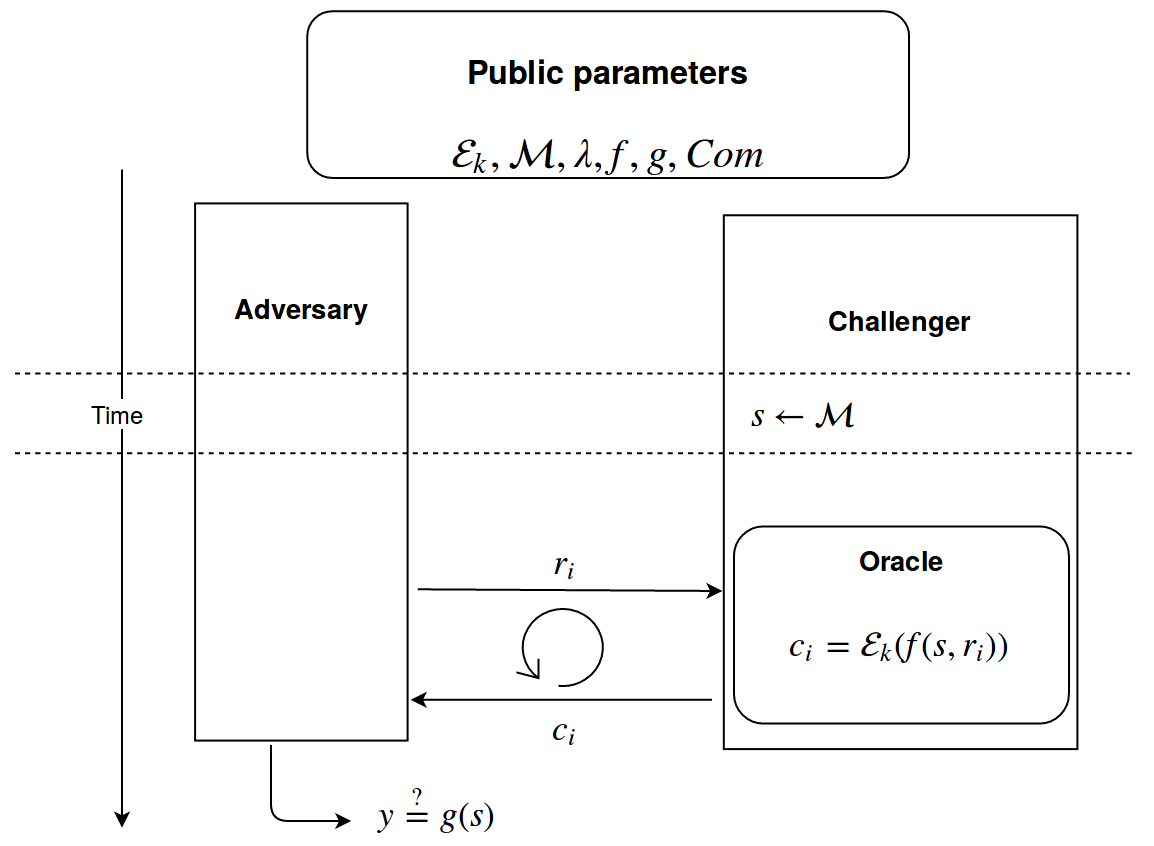
\includegraphics[width=0.48\textwidth]{figures/reflection_game.png}
        \caption{Reflection Game}
        \label{fig:refgame}
    \end{figure}

\subsection{Adversarial advantage}\label{subsec:refsecadv}

Let us now define the advantage of the adversary against a simulator:
\begin{align*}
    \text{Adv}_{\mathcal{SE}, \mathcal{A}, \mathcal{S}}&(\lambda) &\defeq\\
    |\Pr[\text{Game}_{\text{REF-SEC}}^{\mathcal{SE},\mathcal{A}}(\lambda) = 1] &-\\
    \Pr[\text{Game}_{\text{REF-SIM}}^{\mathcal{SE},\mathcal{S}}(\lambda) = 1]| &
\end{align*}

\subsection{Adaptive reflection security}\label{subsec:adaptiverefsec}

Given a rendering function $f(\cdot, \cdot)$, a private-key encryption scheme
$\mathcal{SE}$ composed with a rendering function $f$ is
\textit{reflection-secure} if:
\begin{align*}
    \forall \mathcal{M}:
    \forall g:
    \forall PPT \mathcal{A}:
    \exists PPT \mathcal{S}:\\
    \text{Adv}_{\mathcal{SE}, \mathcal{A}, \mathcal{S}}(\lambda) = negl(\lambda)
\end{align*}

\begin{lemma}[Semantic security]
    Let $(Gen, E, D)$ be a length-preserving reflection-secure encryption
    scheme. Then it is also semantically secure.
\end{lemma}

For a full proof, see Appendix A.
